%!TEX ROOT=main.tex

\section{Soil water content}

Soil is made up of a solid phase of minerals and organic matter, and the pours in-between the solids, which hold gasses and water \cite{paul_soil_2007}. The total amount of moisture is the sum of the moisture contained inside the solids (in intra-aggregate pore space) and the space around the solids (inter-aggregate pore space) \cite{myjove_corporation_determination_2024}. This work will not distinguish between the two for simplicity.

\subsection{Definition}
Soil water or moisture content is a ratio, which ranges from 0, meaning completely dry, to the value of material porosity at saturation \cite{webster_humidity_1998}. It expresses the quantity of water contained in the soil. We can measure it by mass (gravimetric method) or by volume , as depicted in Figure \ref{fig:soil-phase-diagram}.

We can express this mathematically for volumetric content (VWC) as
\begin{equation}
    \label{equation:volumetric-content} \theta = \dfrac{V_w}{V_s + V_w + V_a}
\end{equation}
where $V_w$ is the volume of water and $V_s + V_w + V_a$ is the total volume of the soil sample including contained air. Likewise, gravimetric water content (GWC) is defined as
\begin{equation}
    \label{equation:gravimetric-content} u = \dfrac{m_w}{m_s}
\end{equation}
where $m_w$ is the mass of the water and $m_s$ is mass of all solids in the sample \cite{edaphic_scientific_pty_ltd_how_2024}.

\begin{figure}
    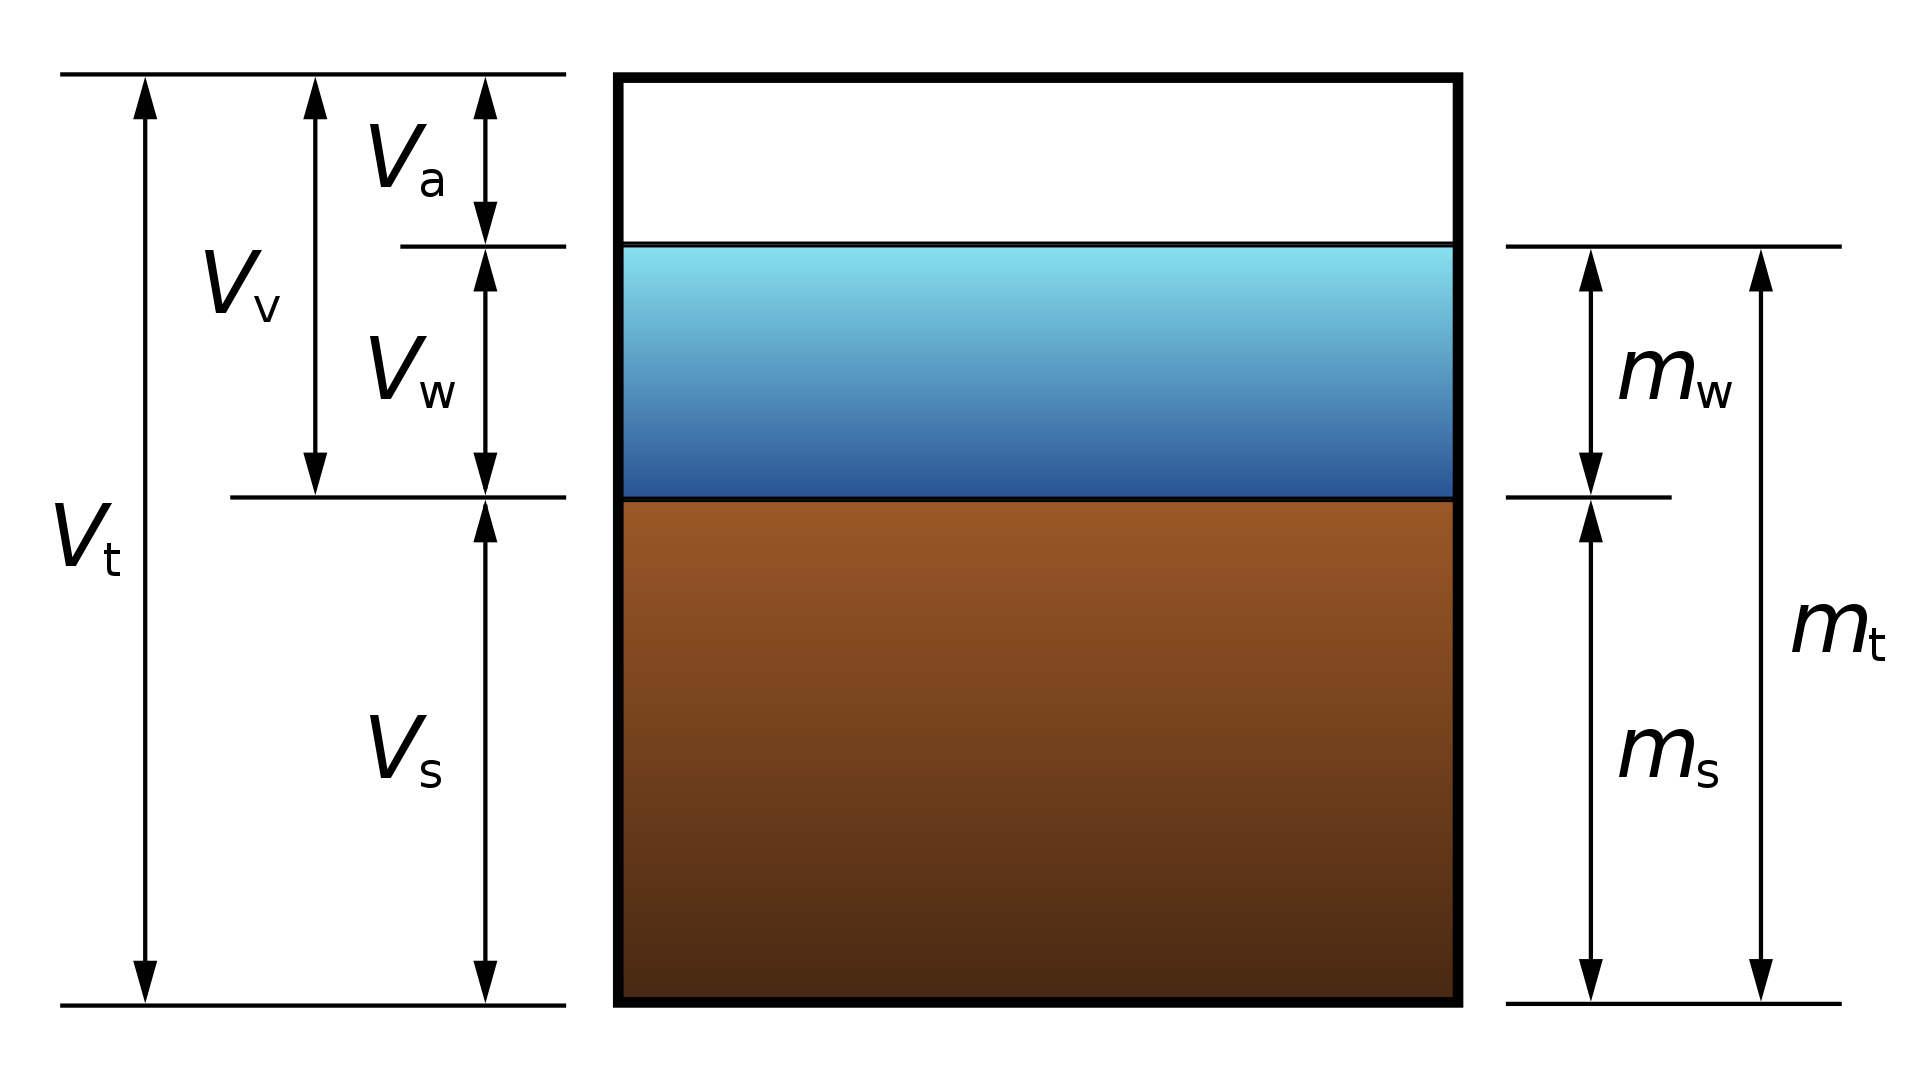
\includegraphics[width=.8\textwidth]{fig/soil-phase-diagram.png}
    \caption{\label{fig:soil-phase-diagram} Soil composition by volume and mass}
    %https://en.wikipedia.org/wiki/Water_content#/media/File:Soil-phase-diagram.svg
\end{figure}

\subsection{Methods of measurement}
\subsubsection{Drying the soil}
Drying the soil sample in a drying oven is a direct method of measurement and is used as the reference method \cite{webster_humidity_1998}. By weighing the sample and also measuring its volume, then doing that again after drying, it is possible to very accurately measure both the volumetric and the gravimetric water content both at the same time.

The procedure involves gathering a known quantity of the sample, ranging from 30 grams to 5 kg, depending on the fines of the particles, heating it up and drying it at 65 to 110 degrees Celsius until the weight stops decreasing \cite{department_of_sustainable_natural_resources_soil_2024,myjove_corporation_determination_2024, paul_soil_2007}.

Since direct methods of measurement of soil moisture content are impractical for field use, we will focus on indirect methods next.

\subsubsection{Geophysical methods}
Geophysical methods exploit other properties of water contained in the soil to approximate the VWC, such as its conductivity, dielectric constant or interaction with neutrons. These methods are thus indirect and subject to inaccuracy if wrong assumptions are used. However, if applied correctly, these methods allow the continuous monitoring of the water content without human intervention. 

\subsubsection{Satellite remote sensing method}
Thanks to recent and ongoing large-scale deployments of Synthetic Aperture Radar satellites, it is possible, that for global-scale soil water content estimation this method will become much more wide-spread. It also relies on the large contrast in dielectric properties of wet and dry soil.

mozna pridat nejakou mapku pro ilustraci?
